% NCVD toolbox user manual.  Compile with XeLaTeX:  latexmk -xelatex NCVD_manual.tex
\documentclass[report]{nld}
\usepackage{amsmath,amsthm}
\usepackage{array,tabularx,longtable}
\usepackage{listings}
\usepackage{subcaption}

\newtheorem{proposition}{Proposition}
\theoremstyle{remark}\newtheorem*{remark}{Remark}

\newcommand{\B}{\mathbf{B}}
\newcommand{\V}{\mathbf{V}}
\newcommand{\T}{\mathbf{T}}
\newcommand{\Y}{\mathbf{Y}}
\newcommand{\X}{\mathbf{X}}
\newcommand{\K}{\mathbf{K}}
\newcommand{\Q}{\mathbf{Q}}
\newcommand{\U}{\mathbf{U}}
\newcommand{\E}{\mathbf{E}}
\newcommand{\R}{\mathbf{R}}
\newcommand{\F}{\mathbf{F}}
\newcommand{\Sg}{\symbf{\Sigma}}
\newcommand{\Lam}{\symbf{\Lambda}}
\newcommand{\Ph}{\symbf{\Phi}}
\newcommand{\Ps}{\symbf{\Psi}}
\newcommand{\Xib}{\symbf{\Xi}}
\renewcommand{\H}{\mathsf{H}}
\newcommand{\code}[1]{\texttt{#1}}
\setlength{\emergencystretch}{3em}

\definecolor{codebg}{HTML}{F1EFE9}
\lstdefinestyle{nld}{basicstyle=\ttfamily\footnotesize, breaklines=true, backgroundcolor=\color{codebg},
  frame=single, rulecolor=\color{nldhairline}, framesep=5pt, xleftmargin=6pt, xrightmargin=6pt,
  keywordstyle=\color{nldnavy}\bfseries, commentstyle=\color{nldmuted}, stringstyle=\color{nldcopperdeep},
  columns=fullflexible, keepspaces=true, showstringspaces=false, upquote=true, aboveskip=0.8em, belowskip=0.8em}
\lstset{style=nld}

\title{NCVD toolbox}
\subtitle{User manual for the Nonlinear Characteristic Value Decomposition\\ in Python and MATLAB, version 1.0}
\reportnumber{User manual}
\author{Nonlinear Dynamics Laboratory}
\date{October 2026}
\runninghead{NCVD toolbox \textperiodcentered{} user manual \textperiodcentered{} github.com/nld-uri/ncvd-toolbox}

\begin{document}
\maketitle
\setcounter{tocdepth}{2}
{\small\tableofcontents}
\newpage

% =====================================================================
\section{Overview}

The NCVD toolbox identifies characteristic values (poles) and characteristic
shapes from a measured or simulated state record. For a record with $n$
stations and $m$ samples it writes
\begin{equation}
  \X_1=[\mathbf{q},\ \dot{\mathbf{q}}]=\U\Ph^\H,\qquad
  \X_2=[\dot{\mathbf{q}},\ \ddot{\mathbf{q}}]=\U\Lam\Ph^\H+\R,\qquad \Lam=\operatorname{diag}(\lambda_i),
  \label{eq:ncvd}
\end{equation}
where $\U$ is the temporal basis, $\Ph$ the characteristic shapes, $\lambda_i$
the characteristic values and $\R$ everything the diagonal form cannot
represent. The first identity is exact. The second is exact for a noise-free
linear record. For noisy, forced or nonlinear data, $\R$ is the least-squares
remainder.

The decomposition descends from the characteristic value decomposition (CVD)
and its generalisation (GCVD) of Li, Stein and Chelidze~\cite{li2025}. It
keeps their data model and quotient but changes how values and shapes are
read out, and it adds the tools a practical identification needs.

\paragraph{What is new relative to the published GCVD.}
\begin{itemize}
  \item \textbf{Exact readout.} The values are the eigenvalues of $\Sg_2$, not
    its diagonal, and the shapes are rotated accordingly. Both identities in
    Eq.~\eqref{eq:ncvd} hold exactly, and $\lambda_i$ belongs to column $i$ of
    $\Ph$ by construction (Section~\ref{sec:algorithm}).
  \item \textbf{Exactness conditions.} Proposition~\ref{prop:exact} states when the
    published diagonal readout is exact and how large its error is when it is
    not (Section~\ref{sec:props}).
  \item \textbf{Time-unit control.} The balanced quotient applies the Joukowski map
    $\lambda\mapsto\tfrac12(\lambda+\lambda^{-1})$, which depends on the unit of
    time. \code{time\_scale='auto'} places every pole where that map is one-to-one
    (Section~\ref{sec:joukowski}).
  \item \textbf{Rates from displacement.} Any FIR derivative stencil, including
    Savitzky--Golay, with exact pole correction (Section~\ref{sec:fir}).
  \item \textbf{Sensor noise.} Least squares (canonical), bias-compensated least
    squares and total least squares (Section~\ref{sec:noise}).
  \item \textbf{Measured forcing}, \textbf{ensembles} of records with different
    sampling rates, \textbf{amplitude tracking} for nonlinear systems, and
    \textbf{reduced-order-model diagnostics} (Sections~\ref{sec:forcing}--\ref{sec:rom}).
\end{itemize}

\paragraph{Where to get it.} Code, manual, slides and animations:
\href{https://github.com/nld-uri/ncvd-toolbox}{\code{github.com/nld-uri/ncvd-toolbox}} (MIT license).
Overview page: \href{https://web.uri.edu/nld/ncvd-toolbox/}{\code{web.uri.edu/nld/ncvd-toolbox}}.

\paragraph{Contents of the toolbox.}
\begin{center}\small
\begin{tabularx}{\linewidth}{@{}>{\raggedright}p{4.3cm}X@{}}
\toprule
Folder & Contents\\
\midrule
\code{python/ncvd/} & Python package (NumPy, SciPy; Matplotlib for figures)\\
\code{python/examples/} & seven worked examples and the paper replication\\
\code{python/tests/} & 28 unit tests, reference copy of the original \code{ncvd.py}\\
\code{matlab/+ncvd/} & MATLAB package, base MATLAB R2022a or later, no toolboxes\\
\code{matlab/examples/}, \code{matlab/tests/} & the same examples; 13 tests including Python cross-checks\\
\code{docs/} & this manual, the slide deck and the animations\\
\bottomrule
\end{tabularx}
\end{center}

\subsection{Quick start}

Python:
\begin{lstlisting}[language=Python]
import numpy as np
import ncvd as nc                                # after: pip install -e python
from ncvd import systems as sy

M, C, K = sy.paper_chain10()                     # 10-DOF chain of [1], App. C.1
t = np.arange(0, 60, 0.05)
d, v, a = sy.simulate_linear(M, C, K, np.random.randn(20), t)

rec = nc.ncvd(d, v, a)                           # X1 = U Phi^H, X2 = U Lam Phi^H + R
mp  = nc.modal_parameters(rec.lam)               # wn, wd, zeta, fn, fd
idx = nc.physical_modes(rec.lam)                 # one pole per conjugate pair
shapes = rec.Psi[:10, idx]                       # displacement part of each mode
print(rec.res, rec.exact1)                       # both ~1e-15 for this record
\end{lstlisting}
MATLAB:
\begin{lstlisting}[language=Matlab]
addpath('path/to/NCVD Toolbox/matlab')
[M, C, K] = ncvd.paperChain10();
t = (0:0.05:60-0.05)';
[d, v, a] = ncvd.simulateLinear(M, C, K, randn(20,1), t);
rec = ncvd.decompose(d, v, a);
mp  = ncvd.modalParameters(rec.lam);
idx = ncvd.physicalModes(rec.lam);
shapes = rec.Psi(1:10, idx);
\end{lstlisting}

\paragraph{Choosing options.}
\begin{center}\small
\begin{tabularx}{\linewidth}{@{}>{\raggedright}p{5.2cm}X@{}}
\toprule
Your data & Use\\
\midrule
Displacement, velocity, acceleration measured or simulated & \code{ncvd(d, v, a)}\\
Displacement only & \code{state\_from\_displacement}, then \code{correct\_poles} (Sec.~\ref{sec:fir})\\
White sensor noise, sampling well above the highest mode & \code{operator='bcls', noise\_var='auto', fs=fs}\\
Measured excitation & \code{forcing=F}\\
Several records, any sampling rates & \code{ncvd\_ensemble(records)}\\
Spectrum spanning decades & \code{rank=r} (whitening)\\
Lightly damped, nondimensional model ($\omega\approx1$) & \code{time\_scale='auto'}\\
Nonlinear free decay & \code{track(d, v, a, fs=..., length=..., step=...)}\\
Multiple equilibria & \code{center=True}\\
\bottomrule
\end{tabularx}
\end{center}

% =====================================================================
\section{The decomposition}\label{sec:decomposition}

\subsection{Data and notation}

$\Y_1,\Y_2\in\mathbb{C}^{m\times p}$ are two records with time along the rows.
For a state record $\Y_1=\X_1=[\mathbf{q},\dot{\mathbf{q}}]$ and
$\Y_2=\X_2=[\dot{\mathbf{q}},\ddot{\mathbf{q}}]$, so $p=2n$. For a linear
system $\dot{\mathbf{x}}=\mathbf{A}\mathbf{x}$ the rows satisfy
$\X_2=\X_1\mathbf{A}^{\mathsf T}$. The second-moment blocks are
$\K_{ij}=\Y_i^\H\Y_j$, and $\B=\Y_1^{\dagger}\Y_2$ is the least-squares
operator of $\Y_2\approx\Y_1\B$. \code{ncvd\_pair(Y1, Y2)} accepts any pair, for
example shift-map or Hankel data; \code{ncvd(d, v, a)} builds the state pair.

\subsection{Algorithm}\label{sec:algorithm}

\begin{enumerate}
  \item \textbf{Preprocess} (optional): remove column means, apply row weights,
    whiten $\Y_1$ to rank $r$, project a measured forcing out of both blocks,
    rescale the time unit used in step~2.
  \item \textbf{Balanced quotient.}
    $\Q=\tfrac14\big(\K_{21}\K_{11}^{-1}+\K_{22}\K_{12}^{-1}+\K_{11}\K_{21}^{-1}+\K_{12}\K_{22}^{-1}\big)$,
    eigenvectors $\V$.
  \item \textbf{Coordinates and coupling.} $\Xib=\Y_1\V^{-\H}$ (so $\Sg_1=\mathbf{I}$)
    and $\Sg_2=\V^{\H}\B\V^{-\H}$.
  \item \textbf{Rotation.} $\Sg_2=\T\Lam\T^{-1}$; $\U=\Xib\T$, $\Ph=\V\T^{-\H}$;
    $\R=\Y_2-\U\Lam\Ph^\H$.
\end{enumerate}
The published GCVD stops after step~3. It returns $\V$ as the shapes and the
diagonal of $\Sg_2$ as the values~\cite[Algorithm~1, Eqs.~(13)--(14)]{li2025}.
Step~4 is the change.

\subsection{Two propositions}\label{sec:props}

\begin{proposition}[Canonical values are least-squares values]\label{prop:ls}
Let $\Q$ and $\Sg_2$ be diagonalisable and $\E=\V^{-\H}\T$. Then $\B\E=\E\Lam$,
$\U=\Y_1\E$ and $\Ph=\E^{-\H}$ for whichever operator $\B$ is used. Hence
$\lambda_i$ are the eigenvalues of $\B$, and the column spaces of $\U$ and
$\Ph$ do not depend on $\Q$; $\Q$ fixes the normalisation of the columns and
the conditioning of the intermediate steps. For the default
\code{operator='ls'} without forcing, $\B=\Y_1^\dagger\Y_2$, so the values are
least-squares values and $\R=(\mathbf{I}-\Y_1\Y_1^\dagger)\Y_2$ (in whitened or
weighted coordinates when \code{rank} or \code{weights} is used).
\end{proposition}
\begin{proof}
$\B\E=\B\V^{-\H}\T=\V^{-\H}\Sg_2\T=\V^{-\H}\T\Lam=\E\Lam$;
$\U=\Y_1\V^{-\H}\T=\Y_1\E$; $\Ph=\V\T^{-\H}=(\T^{-1}\V^\H)^\H=(\E^{-1})^\H$.
Finally $\U\Lam\Ph^\H=\Y_1\E\Lam\E^{-1}=\Y_1\B$.
\end{proof}

For a state record this is the state-variable decomposition with a
least-squares rate model~\cite{feeny2008}, which~\cite{li2025} already
identifies as a special case of CVD. The value of the NCVD formulation lies in
the exact readout, the diagnostics, and the tools of
Sections~\ref{sec:practical}--\ref{sec:nonlinear}, not in a new pole estimator.

\begin{proposition}[When the published readout is exact]\label{prop:exact}
The published readout (values $r_i=(\Sg_2)_{ii}$, shapes $\V$) returns the
eigenvalues of $\B$ together with their eigenvector shapes if and only if
$\Sg_2$ is diagonal, that is, if and only if $\V$ are eigenvectors of $\B^\H$.
(A triangular $\Sg_2$ would still give the right values, but not the right
shapes.) In particular, with $\B$ the least-squares operator:
(i) for the CVD quotient $\K_{21}\K_{11}^{-1}=\B^\H$ and the ``forced''
quotient $\tfrac12(\K_{11}\K_{21}^{-1}+\K_{21}\K_{11}^{-1})=\tfrac12(\B^\H+\B^{-\H})$
it is exact for any data, provided the map separates the eigenvalues;
(ii) for the balanced quotient it is exact when $\Y_2=\Y_1\B$ holds exactly;
(iii) for averaged ensemble quotients and for nonlinear windows it is not exact.
When $\Sg_2=\mathbf{D}+\mathbf{F}$ with $\mathbf{F}$ off-diagonal, the diagonal
readout's pole error is $O(\|\mathbf{F}\|^2/\delta)$ and its shape error is
$O(\|\mathbf{F}\|/\delta)$, where $\delta$ is the eigenvalue gap (first-order
perturbation theory; fitted slopes 1.74 and 1.05 in Example~7).
\end{proposition}

\begin{proof}
If $\B^\H\V=\V\mathbf{D}$ then $\V^\H\B=\mathbf{D}^\H\V^\H$ and $\Sg_2=\mathbf{D}^\H$,
which is diagonal; conversely, a diagonal $\Sg_2$ means $\B\V^{-\H}=\V^{-\H}\Sg_2$.
For (i), $\K_{21}\K_{11}^{-1}=(\K_{11}^{-1}\K_{12})^\H=\B^\H$, so both quotients are
functions $f(\B^\H)$; when $f$ separates the eigenvalues, their eigenvectors are
those of $\B^\H$. For (ii), $\K_{12}\K_{22}^{-1}=\B_b^\H$ with $\B_b=\Y_2^\dagger\Y_1$,
and $\B_b=\B^{-1}$ exactly when $\Y_2=\Y_1\B$. The orders follow from first-order
perturbation of a diagonal matrix by an off-diagonal one, which leaves the
diagonal unchanged.
\end{proof}

\code{python/examples/paper\_replication.py} reruns every experiment
of~\cite{li2025} with both readouts. The published results do not change: the
experiments there satisfy (i) or (ii). Figure~\ref{fig:readout} shows both
failure modes.

\begin{figure}[h]
  \centering
  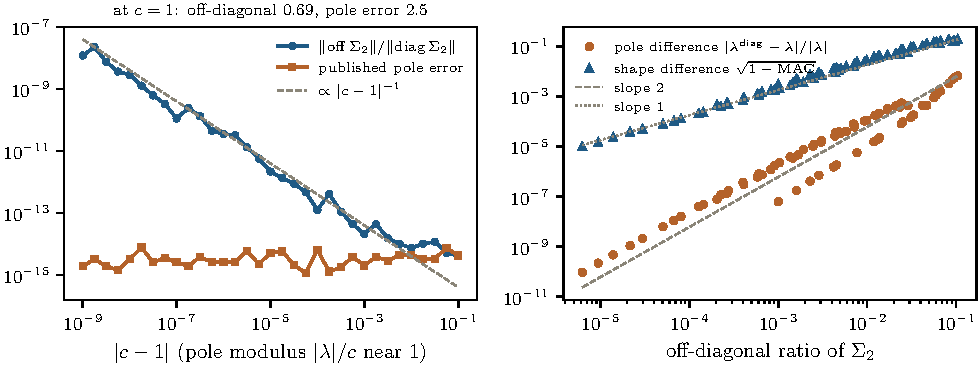
\includegraphics[width=\linewidth]{figures/ex07_readout_error.pdf}
  \caption{Published against canonical readout. (a) A lightly damped chain
  with $\omega=1$, time unit scaled by $c$; at $c=1$ a pole meets its conjugate
  under the balanced map. (b) Windows of a nonlinear decay: pole difference of
  second order, shape difference of first order in the off-diagonal ratio of
  $\Sg_2$ (fitted slopes 1.74 and 1.05). Example~7.}
  \label{fig:readout}
\end{figure}

\subsection{Geometry}\label{sec:geometry}

Three pictures carry most of the intuition. Each has an animated version in
\code{docs/animations/} and in the slide deck.

\paragraph{The residual is a projection.} Each column of $\X_2$ is split into
its orthogonal projection on the column space of $\X_1$, which the diagonal
form reproduces exactly, and a remainder orthogonal to it
(Figure~\ref{fig:geom}a). For a noise-free linear record the remainder is zero.
For a window of a nonlinear decay, $\|\R\|/\|\X_2\|$ measures the part of the
rate data that no linear model of that window explains.

\paragraph{A complex mode is a rotating, shrinking polygon.} With non-proportional
damping the eigenvector $\psi$ has entries with different phases. The modal
contribution $\psi_j e^{\lambda t}$ of each station is a phasor; together they
form a polygon that rotates at $\operatorname{Im}\lambda$ and shrinks at
$\operatorname{Re}\lambda$. The motion is its real part, and the nodes
travel. The modal phase collinearity
(MPC)~\cite{li2025} measures how close the polygon is to a line
(Figure~\ref{fig:geom}b).

\paragraph{The balanced quotient folds the plane.} For exact linear data,
$\Q=\tfrac12(\mathbf{A}+\mathbf{A}^{-1})$, so its eigenvalues are
$\mu=\tfrac12(\lambda+\lambda^{-1})$. This Joukowski map is one-to-one outside
(or inside) the unit circle, but it sends $\lambda$ and $1/\lambda$ to the same
point and squeezes the unit circle onto $[-1,1]$. A pole with $|\lambda|=1$ in
the chosen time unit meets its conjugate (Figure~\ref{fig:geom}c). Rescaling
time moves the poles relative to the circle; see Section~\ref{sec:joukowski}.

\begin{figure}[p]
  \centering
  \begin{subfigure}{\linewidth}\centering
    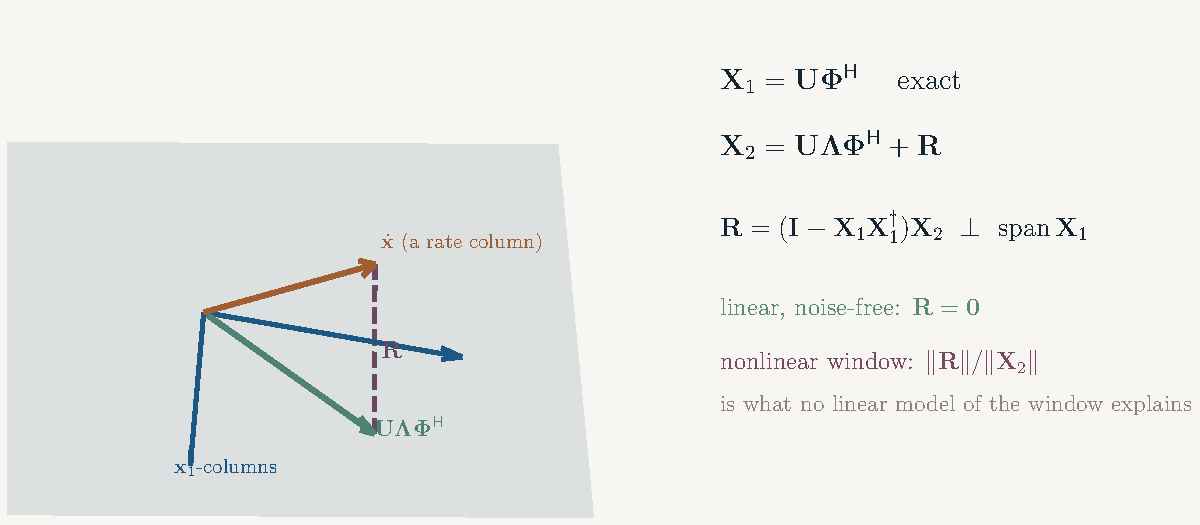
\includegraphics[width=0.95\linewidth]{figures/residual_projection_still.pdf}
    \caption{The fit is the projection of each rate column on $\operatorname{span}\X_1$; $\R$ is orthogonal to it.}
  \end{subfigure}\\[0.6em]
  \begin{subfigure}{\linewidth}\centering
    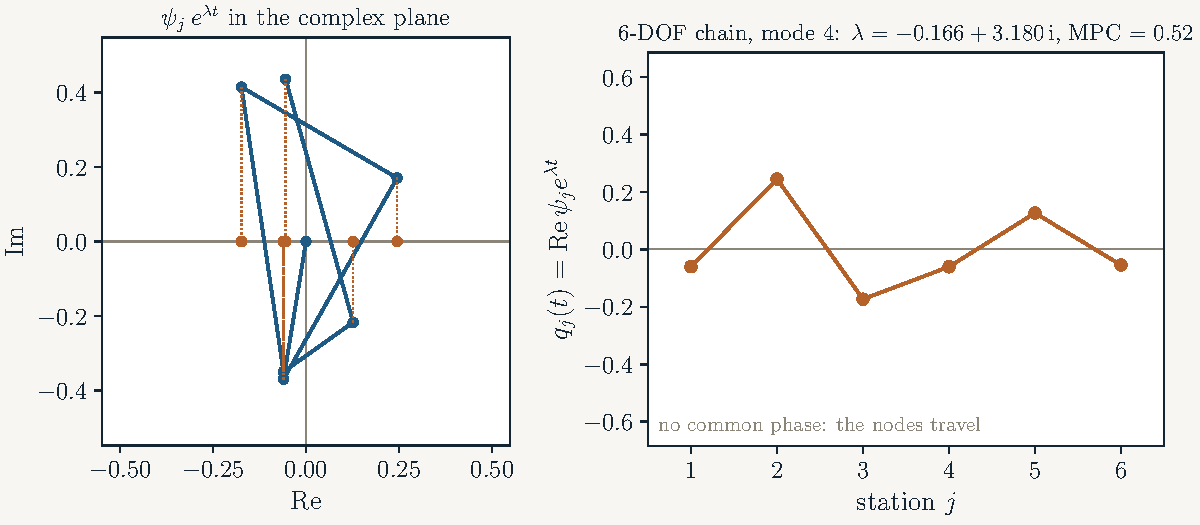
\includegraphics[width=0.95\linewidth]{figures/complex_mode_still.pdf}
    \caption{Mode 4 of a 6-DOF chain with dampers at the first two masses (MPC $=0.52$).}
  \end{subfigure}\\[0.6em]
  \begin{subfigure}{\linewidth}\centering
    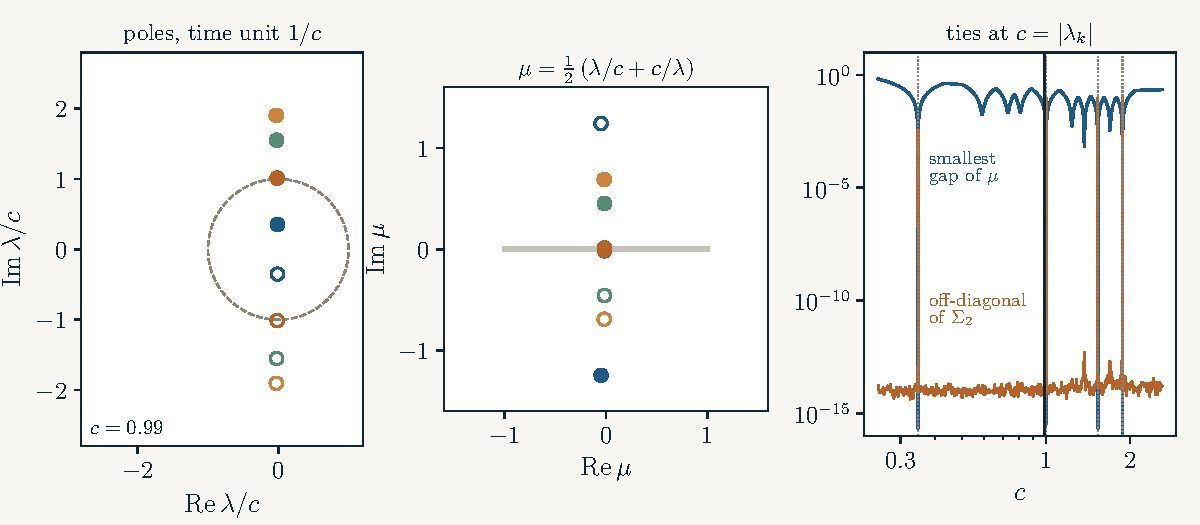
\includegraphics[width=0.95\linewidth]{figures/joukowski_fold_still.pdf}
    \caption{Poles $\lambda/c$, their images $\mu$, and the minimum gap of $\mu$ and the
    off-diagonal ratio of $\Sg_2$ against $c$ for a 4-DOF chain with $\omega_2=1$.}
  \end{subfigure}
  \caption{Three geometric pictures (stills of the animations).}
  \label{fig:geom}
\end{figure}

\subsection{Conventions}

\begin{itemize}
  \item \textbf{$\Ph$ and $\Ps$.} $\X_1=\U\Ph^\H$ gives
    $\mathbf{x}(t)=\sum_i u_i(t)\,\overline{\symbf{\phi}_i}$. The eigenvector of $\mathbf{A}$
    for $\lambda_i$ is therefore $\psi_i=\overline{\symbf{\phi}_i}$, returned as \code{Psi}.
    Compare shapes with \code{Psi}; its velocity half equals $\lambda_i$ times
    its displacement half for a linear record.
  \item \textbf{Order.} By default, modes are sorted by ascending
    $|\operatorname{Im}\lambda|$, positive imaginary part first in each pair,
    real poles last. \code{physical\_modes} returns one index per pair.
  \item \textbf{Units.} $\lambda$ is in rad per time unit of the data.
    \code{modal\_parameters} returns $\omega_n=|\lambda|$,
    $\omega_d=|\operatorname{Im}\lambda|$, $\zeta=-\operatorname{Re}\lambda/|\lambda|$,
    and the same in cycles.
\end{itemize}

% =====================================================================
\section{Practical data}\label{sec:practical}

\subsection{Rates from displacement}\label{sec:fir}

If velocity and acceleration are produced by one linear, shift-invariant FIR
stencil $D$, with $(D\mathbf{q})_k=f_s\sum_j c_j\mathbf{q}_{k+j}$, applied
consistently,
$\X_1=[\mathbf{q},D\mathbf{q}]$ and $\X_2=[D\mathbf{q},DD\mathbf{q}]$, then a free (unforced)
linear record still satisfies $\X_2=\X_1\tilde{\mathbf{A}}^{\mathsf T}$ exactly. Here
$\tilde{\mathbf{A}}$ has the eigenvectors $[\psi;\,d(\theta)\psi]$, whose
displacement half $\psi$ is that of $\mathbf{A}$, and the eigenvalues
\begin{equation}
  \tilde\lambda=d(\theta),\qquad \theta=e^{\lambda\Delta t},\qquad d(\theta)=f_s\sum_j c_j\theta^{j}.
\end{equation}
The NCVD therefore returns $d(\theta)$. \code{correct\_poles} solves
$d(\theta)=\tilde\lambda$, keeps the root with the smallest $|\log\theta|$, and
returns $f_s\log\theta$. For the forward difference this is Eq.~(48)
of~\cite{li2025}. The displacement half of each shape is unaffected.

The inversion is unique only where the stencil's symbol is one-to-one along
the unit circle. Central-type stencils turn over: $\omega\Delta t$ and
$\pi-\omega\Delta t$ give the same central difference. \code{band()}
(MATLAB \code{filterBand}) returns the limit.

\begin{center}\footnotesize\setlength{\tabcolsep}{4pt}
\begin{tabular}{@{}lccc@{}}
\toprule
Stencil & \code{method} & Band $\omega\Delta t<$ & Error in band (Ex.~2)\\
\midrule
forward / backward & \code{'forward'}, \code{'backward'} & $\pi$ & $4.4\times10^{-14}$\\
central & \code{'central'} & $\pi/2$ & $7.0\times10^{-14}$\\
five-point central & \code{'central4'} & 1.798 & $7.2\times10^{-13}$\\
Savitzky--Golay (7, 3)~\cite{savitzky1964} & \code{'savgol'} & 1.141 & $3.0\times10^{-13}$\\
\bottomrule
\end{tabular}
\end{center}

\begin{lstlisting}[language=Python]
d, v, a, filt, k0 = nc.state_from_displacement(q, fs, 'savgol', window=7, polyorder=3)
rec = nc.ncvd(d, v, a)
lam = nc.correct_poles(rec.lam, filt, fs)        # then re-sort if needed
assert np.all(np.abs(lam.imag)/fs < filt.band())
\end{lstlisting}

\begin{figure}[h]
  \centering
  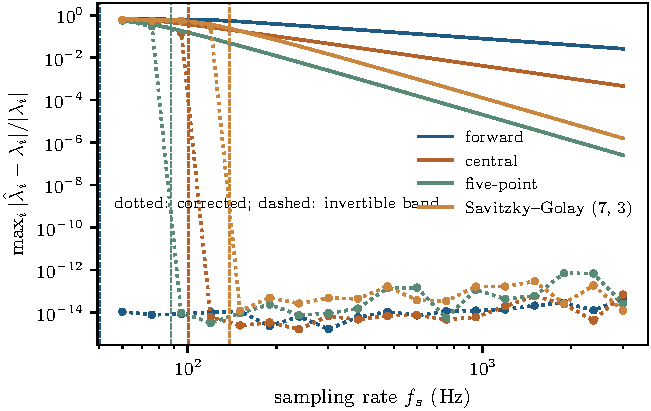
\includegraphics[width=0.62\linewidth]{figures/ex02_fd_correction.pdf}\hfill
  \caption{Example 2: 3-DOF chain of~\cite[App.~C.2]{li2025} (4.24, 70.7 and
  158 rad/s). Solid: raw poles from FIR rates. Dotted: after
  \code{correct\_poles}, at machine precision to the left of each stencil's band
  limit (dashed).}
  \label{fig:fir}
\end{figure}

\subsection{Sensor noise}\label{sec:noise}

By Proposition~\ref{prop:ls}, the canonical values are least-squares values.
White noise in the regressors $\Y_1$ adds $m\,\mathbf{N}$ to $\K_{11}$, with
$\mathbf{N}$ the noise covariance, and biases $\B$ toward zero. This is the
classical errors-in-variables bias~\cite{soderstrom2007}. Three operators are
available:
\begin{itemize}
  \item \code{'ls'} (default): $\B=\Y_1^\dagger\Y_2$. Exact for clean data,
    consistent for noise in $\Y_2$ only, and for unmeasured forcing
    uncorrelated with the present state.
  \item \code{'bcls'}: $\B=(\K_{11}-m\mathbf{N})^{-1}\K_{12}$, with only the
    acceleration block regressed so that $\dot{\mathbf{q}}=\dot{\mathbf{q}}$ stays
    exact. \code{noise\_var='auto'} estimates $\mathbf{N}$ per channel from the
    flat spectrum between $0.40f_s$ and $0.49f_s$. This needs a sampling rate
    well above the highest mode.
  \item \code{'tls'}: total least squares~\cite{golub1980} on column-equilibrated
    data. Use it only for free decays with measurement noise. Under unmeasured
    forcing it treats the force as noise, and it fails (Figure~\ref{fig:noise}).
\end{itemize}

\begin{figure}[h]
  \centering
  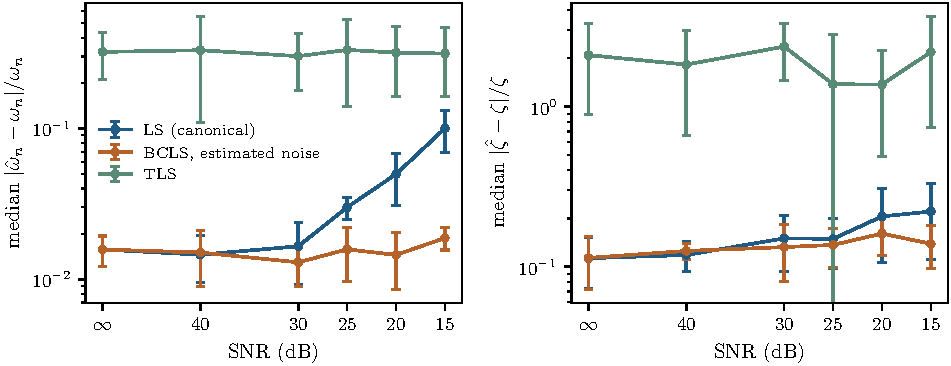
\includegraphics[width=\linewidth]{figures/ex03_noise_operators.pdf}
  \caption{Example 3: the 10-DOF chain under unmeasured white forcing at every
  mass, 200 Hz for 150 s, independent noise on every channel; mean and spread
  over 10 records. From $\infty$ to 15 dB the median frequency error grows from
  1.6\,\% to 10\,\% with \code{'ls'} and stays below 1.9\,\% with
  \code{'bcls'}. The remaining damping error (about 11--16\,\%) is the
  statistical error of a finite record under random forcing.}
  \label{fig:noise}
\end{figure}

\subsection{Measured forcing}\label{sec:forcing}

With a measured input record $\F$ ($m\times q$), \code{forcing=F} projects $\F$
out of both blocks before the operator is estimated (Frisch--Waugh), and
returns the input gains as \code{G}. No mass matrix or input matrix is needed.
On the 4-DOF chain of Example~6, driven at three of four masses, the pole
error is $2.7\times10^{-15}$ with the forcing and $4.8\times10^{-2}$ without.
This replaces Eq.~(41) of~\cite{li2025}, which requires the forcing in state
space and therefore the mass matrix.

For unmeasured random forcing (operational modal analysis), the default
operator is the forward regression of $\X_2$ on $\X_1$. It does not use $\K_{22}$,
whose forcing autocovariance biases the four-term balanced
quotient~\cite[Sec.~5.3]{li2025}.

\subsection{Ensembles}\label{sec:ensemble}

The state-rate relation is continuous-time, so records with different sampling
rates, lengths and noise levels share one operator. \code{ncvd\_ensemble}
stacks their rows and decomposes once; this is the least-squares fusion of all
records. Weights are \code{'equal'} (default, every record counts equally),
\code{'samples'}, \code{'snr'} (weight $1/(m_i\,\hat\sigma_i^2)$ with
$\hat\sigma_i^2$ the relative residual variance of record $i$), or a vector.
\code{rec.blocks[i]} gives each record's rows of $\U$. For the 16 trials of
Table~5 of~\cite{li2025} (Example~4), the mean frequency error falls from
1.5\,\% (one trial) to 0.34\,\% (16), and the shape error from 0.23 to 0.074.

\begin{figure}[h]
  \centering
  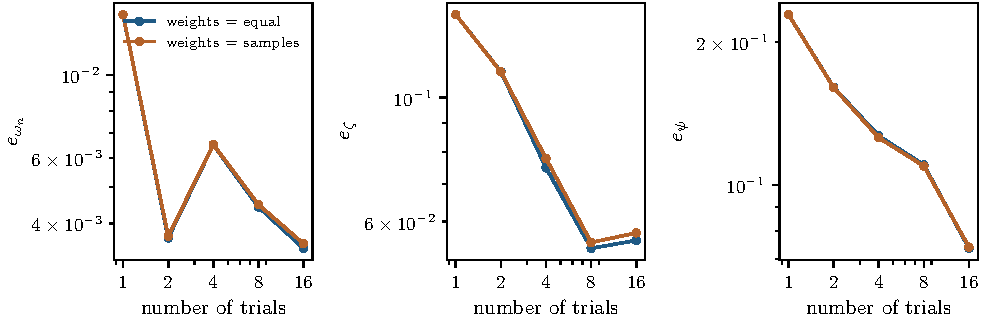
\includegraphics[width=\linewidth]{figures/ex04_ensemble.pdf}
  \caption{Example 4: ensemble errors against the number of trials.}
\end{figure}

\subsection{Time units, conditioning and rank}\label{sec:joukowski}

The values do not depend on the time unit, but the balanced quotient does
(Section~\ref{sec:geometry}). \code{time\_scale=c} measures time in units of
$1/c$ while forming $\Q$; \code{'auto'} chooses $c=\min|\lambda_{\mathrm{LS}}|/2$
so that every pole has modulus at least 2, where the Joukowski map is
one-to-one. With the canonical readout the values are exact either way.
The option makes $\V$ nearly diagonalise $\Sg_2$ (\code{condT} close to 1),
which keeps the intermediate steps well conditioned and makes the published
and canonical readouts agree. \code{track} uses \code{'auto'} by default.

\code{rank=r} whitens $\Y_1$ by its SVD before decomposing. It does not change
the values when $\Y_1$ has full column rank. It repairs conditioning when the
spectrum spans decades or when stations are redundant. Shapes are mapped back
to the original coordinates.

% =====================================================================
\section{Nonlinear systems}\label{sec:nonlinear}

\subsection{Sliding windows}

A nonlinear free decay passes through a sequence of energy levels. Each short
window is decomposed. Its values are the best linear description of the local
dynamics, and following each resonance through the windows traces its
frequency-energy dependence: the data-driven counterpart of a nonlinear normal
mode backbone curve~\cite{stein2025}.

\begin{lstlisting}[language=Python]
tr = nc.track(d, v, a, fs=fs, length=800, step=400, n_track=3, M=M)
tr.wd, tr.zeta, tr.energy, tr.shape, tr.mpc, tr.res      # per window and mode
f1 = [nc.band_frequency(d[s:e, 0], 1/fs, 0.6, 1.1) for s, e in tr.edges]
\end{lstlisting}
Consecutive windows are matched by minimising $(1-\mathrm{MAC})+|\log(\omega/\omega_{\mathrm{prev}})|$
as an assignment problem. With a mass matrix, \code{amp} and \code{energy}
are mass-normalised modal amplitude and energy.

\begin{figure}[h]
  \centering
  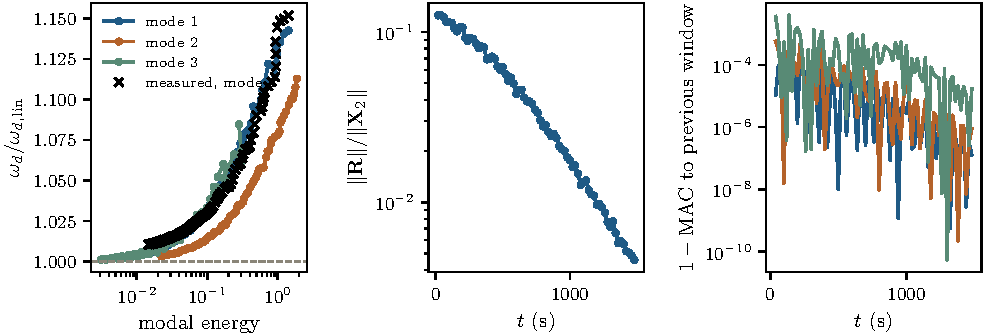
\includegraphics[width=\linewidth]{figures/ex05_duffing_backbone.pdf}
  \caption{Example 5: 3-DOF chain with a cubic spring ($k_3=1$) grounding the
  first mass, damping $0.003\mathbf{M}$, one free decay of 1500 s, windows of
  40 s every 20 s. Left: damped frequency against modal energy, normalised by
  the linear value; crosses are the measured response frequency of mode~1 in
  each window (largest difference 1.5\,\%). Centre: window residual. Right:
  shape change between consecutive windows.}
  \label{fig:backbone}
\end{figure}

\subsection{Requirements and caveats}

\begin{itemize}
  \item \textbf{Excite every resonance you track.} A release along one mode makes
    the record rank deficient. Check the singular values \code{rec.s} of each window.
  \item \textbf{Each window must span at least one period of the slowest mode.}
    A dozen periods determine the pole well. Shorter windows resolve faster
    amplitude changes at the cost of scatter.
  \item \textbf{Weak modes lose their pole slot.} A window of a $2n$-dimensional
    record has $2n$ poles. If a resonance carries less energy than a
    superharmonic of a strong one, the superharmonic takes its slot. In our run
    of the Duffing chain of Example~5 with stiffness-proportional damping
    ($\mathbf{C}=0.004\,\mathbf{K}$), mode 3 decayed early and its slot drifted
    to $3\omega_1$. Watch for a ``mode'' whose frequency
    approaches a multiple of another.
  \item \textbf{Validate every pole} against the measured response frequency
    (\code{band\_frequency}); the comparison shows where the linear-pole
    description of a window holds.
  \item \textbf{Damping from single nonlinear windows scatters.} It can come out
    negative on a decaying record. Frequencies and shapes are the reliable outputs.
  \item \textbf{\code{center=True}} (the default in \code{track}) is needed whenever
    the motion is not about the origin.
  \item \textbf{The residual} \code{tr.res} is an indicator of how strongly
    each window engages the nonlinearity (and noise). It is not a calibrated measure.
\end{itemize}

\subsection{Reduced-order-model diagnostics}\label{sec:rom}

The \code{rom} module works with the family of shapes one resonance takes over
the swept energy range~\cite{stein2025}:
\code{robustness\_basis} (SVD of the family), \code{deflate} (near-linear shape
$\mathbf{v}_0$, leading amplitude correction and its relative size),
\code{escape} (the part of each correction outside a retained span),
\code{closure} (smallest retained set that contains the first $k$ corrections)
and \code{project} (Galerkin projection of $\mathbf{M}$, $\mathbf{K}$, $\mathbf{C}$
and the nonlinear force).

\begin{remark}
These quantities are built from differences of shapes. By
Proposition~\ref{prop:exact}, shapes from the superseded diagonal readout
differ from the canonical shapes at first order in the off-diagonal part of
$\Sg_2$. Values of corrections, escape and closure computed with the two
readouts can therefore differ much more than the shapes do, and must not be
mixed.
\end{remark}

% =====================================================================
\section{Reference}\label{sec:reference}

\subsection{Installation}

Clone \code{https://github.com/nld-uri/ncvd-toolbox}. Python 3.9 or later: \code{pip install -e python} (add \code{[plot,test]} for
figures and tests); \code{python -m pytest -q} in \code{python/}. MATLAB
R2022a or later: \code{addpath('.../matlab')};
\code{runtests('tests/test\_ncvd.m')} in \code{matlab/}; \code{help ncvd} lists
every function. Figures use LaTeX text: in Python \code{plotting.set\_style()}
(needs a TeX installation with \code{cm-super}), in MATLAB \code{ncvd.setStyle()}.

\subsection{Functions}

\begin{center}\small
\begin{longtable}{@{}>{\raggedright}p{4.6cm}>{\raggedright}p{4.4cm}>{\raggedright\arraybackslash}p{6.2cm}@{}}
\toprule
Python (\code{import ncvd as nc}) & MATLAB (\code{ncvd.*}) & Purpose\\
\midrule\endhead
\code{ncvd(d, v, a, ...)} & \code{decompose(d, v, a, ...)} & canonical NCVD of a state record\\
\code{ncvd\_pair(Y1, Y2, ...)} & \code{decomposePair(Y1, Y2, ...)} & any pair, $\Y_2\approx\Y_1\B$\\
\code{balanced\_quotient} & \code{balancedQuotient} & $\Q$\\
\code{regression\_operator} & \code{regressionOperator} & LS, TLS, BCLS operator\\
\code{auto\_time\_scale} & \code{autoTimeScale} & time unit for an injective balanced map\\
\code{noise\_variance} & \code{noiseVariance} & per-channel noise variance near Nyquist\\
\code{modal\_parameters} & \code{modalParameters} & $\omega_n$, $\omega_d$, $\zeta$, $f_n$, $f_d$\\
\code{physical\_modes} & \code{physicalModes} & one index per conjugate pair\\
\code{realify} & \code{realify} & real shape and MPC\\
\code{mac}, \code{mac\_matrix} & \code{mac}, \code{macMatrix} & modal assurance criterion\\
\code{mac\_phase\_matched} & \code{macPhaseMatched} & MAC after Eq.~(55) of~\cite{li2025}\\
\code{relative\_error} & \code{relativeError} & Eq.~(56) of~\cite{li2025}\\
\code{match\_modes} & \code{matchModes} & one-to-one matching to reference modes\\
\code{deriv\_filter}, \code{DerivFilter.band} & \code{derivFilter}, \code{filterBand} & FIR stencils and their bands\\
\code{state\_from\_displacement} & \code{stateFromDisplacement} & consistent $(\mathbf{q},D\mathbf{q},DD\mathbf{q})$\\
\code{correct\_poles} & \code{correctPoles} & exact FIR pole correction\\
\code{track}, \code{window\_edges} & \code{track}, \code{windowEdges} & sliding windows and tracking\\
\code{band\_frequency} & \code{bandFrequency} & measured frequency for validation\\
\code{ncvd\_ensemble} & \code{ensemble} & joint NCVD of several records\\
\code{rom.robustness\_basis}, \code{rom.deflate}, \code{rom.escape}, \code{rom.closure}, \code{rom.project} & \code{robustnessBasis}, \code{deflate}, \code{escape}, \code{closure}, \code{project} & ROM diagnostics\\
\code{benchmarks.gcvd}, \code{.dmd}, \code{.itd} & \code{gcvd}, \code{dmd}, \code{itd} & published GCVD readout, DMD~\cite{schmid2010}, ITD~\cite{ibrahim1982}\\
\code{systems.*} & \code{chain}, \code{paperChain10}, \dots & test systems, simulation, noise\\
\code{plotting.set\_style} & \code{setStyle} & LaTeX text and palettes\\
\bottomrule
\end{longtable}
\end{center}

\subsection{Options of \code{ncvd} / \code{decompose}}

\begin{center}\small
\begin{tabularx}{\linewidth}{@{}>{\raggedright}p{3.4cm}>{\raggedright}p{2.4cm}X@{}}
\toprule
Python / MATLAB & Default & Meaning\\
\midrule
\code{rank} / \code{Rank} & none & whiten $\Y_1$ to this rank\\
\code{center} / \code{Center} & false & remove column means\\
\code{operator} / \code{Operator} & \code{'ls'} & \code{'ls'}, \code{'tls'}, \code{'bcls'}\\
\code{noise\_var}, \code{fs} / \code{NoiseVar}, \code{Fs} & none & noise variances of $[\mathbf{q},\dot{\mathbf{q}}]$ or \code{'auto'} (BCLS)\\
\code{forcing} / \code{Forcing} & none & measured input record, $m\times q$\\
\code{time\_scale} / \code{TimeScale} & none & number $c$ or \code{'auto'}\\
\code{weights} / \code{Weights} & none & row weights\\
\code{sort} / \code{Sort} & true & order by $|\operatorname{Im}\lambda|$\\
\code{structured} / \code{Structured} & true & keep the kinematic block exact in TLS/BCLS\\
\code{readout} / \code{Readout} & \code{'eig'} & \code{'diag'} gives the published readout (benchmarking)\\
\code{legacy\_balanced} / \code{LegacyBalanced} & false & superseded shapes with assignment heuristic\\
\bottomrule
\end{tabularx}
\end{center}

\subsection{Result fields}

\begin{center}\small
\begin{tabularx}{\linewidth}{@{}>{\raggedright}p{2.8cm}X@{}}
\toprule
Field & Meaning\\
\midrule
\code{lam} & characteristic values, $\lambda_i$ paired with column $i$\\
\code{Phi}, \code{Psi} & regression shapes ($\X_1=\U\Ph^\H$) and eigenvector shapes $\Ps=\overline{\Ph}$\\
\code{U} & temporal basis\\
\code{R} & residual of the second identity (whitened coordinates if \code{rank})\\
\code{res}, \code{exact1} & $\|\R\|/\|\X_2\|$ and $\|\X_1-\U\Ph^\H\|/\|\X_1\|$\\
\code{resid} & relative least-squares residual of $\X_2$ on $\X_1$\\
\code{V}, \code{T}, \code{S2}, \code{B} & balanced eigenvectors, rotation, $\Sg_2$, operator\\
\code{condT}, \code{condV} & condition numbers of $\T$ and $\V$\\
\code{s} & singular values of $\X_1$\\
\code{G} & input gains (with forcing)\\
\code{share} & pole-to-shape weight (1 except for the legacy readout)\\
\code{time\_scale}, \code{operator}, \code{readout} & options used (MATLAB: \code{timeScale})\\
\bottomrule
\end{tabularx}
\end{center}

% =====================================================================
\section{Validation}

\begin{itemize}
  \item \textbf{Python, 28 tests}: reproduction of the original \code{ncvd.py}
    to $10^{-10}$ (values) and $10^{-8}$ (shapes, coordinates), with and
    without whitening and the legacy readout; identities and poles to
    $10^{-9}$ or better; Propositions~\ref{prop:ls} and~\ref{prop:exact};
    time-unit invariance; FIR correction for five stencils; forcing; ensembles;
    DMD and ITD on clean data; tracking on linear and Duffing records; BCLS
    bias reduction; ROM helpers.
  \item \textbf{MATLAB, 13 tests}, run on R2026b: the same checks, plus
    cross-checks against stored Python results: clean values to $10^{-10}$,
    noisy values to $10^{-9}$ (LS), $10^{-8}$ (BCLS, diagonal readout, whitening)
    and $10^{-7}$ (TLS), the noise estimate to $10^{-8}$, FIR correction, tracking to
    $10^{-8}$, and the Duffing simulation to $10^{-6}$.
  \item \textbf{Replication of~\cite{li2025}}
    (\code{python/examples/paper\_replication.py}): the published and canonical
    readouts agree to $10^{-14}$ on the single-record noise study and the
    undersampling study. They differ by at most 0.5\,\% in individual poles on
    the ensemble study, with mode-averaged errors unchanged in trend.
\end{itemize}

\section{Limitations}

\begin{itemize}
  \item The values are least-squares values (Proposition~\ref{prop:ls}). Under
    random forcing with a finite record, the damping error is statistical, about
    11--22\,\% in Example~3, and no readout removes it.
  \item BCLS assumes white sensor noise, independent between channels, and a
    noise-only band near Nyquist. Coloured noise, or noise from differentiating
    a noisy displacement, violates both assumptions.
  \item The FIR correction assumes the same stencil for both derivatives and
    holds only inside the stencil's band.
  \item Windowed values of nonlinear systems are equivalent-linear values of
    the window. Their meaning degrades with orbit anharmonicity and where
    another mode or a superharmonic dominates the window.
  \item Exact Joukowski ties (Section~\ref{sec:joukowski}) affect only the
    published readout and the conditioning of $\V$, never the canonical values.
\end{itemize}

\begin{thebibliography}{9}\small
\bibitem{li2025} H.-W.-X. Li, D.~L. Stein, D.~Chelidze, Characteristic value
  decomposition: A unifying paradigm for data-driven modal analysis,
  \emph{Mechanical Systems and Signal Processing} 222 (2025) 111769,
  doi:10.1016/j.ymssp.2024.111769.
\bibitem{stein2025} D.~L. Stein, D.~Chelidze, Continuation of nonlinear normal
  modes using reduced-order models based on generalized characteristic value
  decomposition, \emph{Nonlinear Dynamics} 113 (2025) 25--45,
  doi:10.1007/s11071-024-10239-0.
\bibitem{feeny2008} B.~F. Feeny, U.~Farooq, A nonsymmetric state-variable
  decomposition for modal analysis, \emph{Journal of Sound and Vibration} 310 (4)
  (2008) 792--800, doi:10.1016/j.jsv.2007.11.012.
\bibitem{savitzky1964} A.~Savitzky, M.~J.~E. Golay, Smoothing and
  differentiation of data by simplified least squares procedures,
  \emph{Analytical Chemistry} 36 (8) (1964) 1627--1639, doi:10.1021/ac60214a047.
\bibitem{golub1980} G.~H. Golub, C.~F. Van~Loan, An analysis of the total least
  squares problem, \emph{SIAM Journal on Numerical Analysis} 17 (6) (1980)
  883--893, doi:10.1137/0717073.
\bibitem{soderstrom2007} T.~S\"oderstr\"om, Errors-in-variables methods in
  system identification, \emph{Automatica} 43 (6) (2007) 939--958,
  doi:10.1016/j.automatica.2006.11.025.
\bibitem{schmid2010} P.~J. Schmid, Dynamic mode decomposition of numerical and
  experimental data, \emph{Journal of Fluid Mechanics} 656 (2010) 5--28,
  doi:10.1017/S0022112010001217.
\bibitem{ibrahim1982} S.~R. Ibrahim, R.~S. Pappa, Large modal survey testing
  using the Ibrahim time domain identification technique, \emph{Journal of
  Spacecraft and Rockets} 19 (5) (1982) 459--465, doi:10.2514/3.62285.
\end{thebibliography}

\end{document}
